\section{Comparison with the state of the art}
\label{sec:results}

\ifpreliminary
\noindent\fcolorbox{red!60!black}{red!5}{%
\begin{minipage}{0.955\columnwidth}\footnotesize
\textbf{Status of this section.} Tables~\ref{tab:baselines} and~\ref{tab:panelb} were
both regenerated from HEAD (Panel A: 2026-08-31, Panel B: 2026-08-30; see
\texttt{paper/PROVENANCE.md} for commit hashes and per-artifact provenance) and the TGN
row of Table~\ref{tab:baselines} now runs under the same deployable protocol as every
baseline row.
This box only renders while \texttt{main.tex} carries \texttt{\textbackslash
preliminarytrue}; at time of writing that flag is false and it is not shown.
\end{minipage}}
\vspace{2mm}
\fi

\subsection{Qualitative positioning}

\begin{table*}[ht!]
\centering
\renewcommand{\arraystretch}{1.5}
\footnotesize
\setlength{\tabcolsep}{3pt}
\begin{tabular}{lccccccc}
\toprule
& \textit{Euler}~\cite{euler} & \textit{Argus}~\cite{argus} & \textit{LMDetect}~\cite{lmdetect} & GFM~\cite{gfm} & Static GNN & IF / OC-SVM & \textit{This work} \\
\midrule
Substrate            & auth log & auth log & auth log & auth log & ZTA stream & ZTA stream & \textit{ZTA request stream} \\
Node types           & host & host & host, user & host, user & 5 & --- (tabular) & \textit{5, incl.\ client config} \\
Client fingerprint node & no & no & no & no & yes & --- & \textit{yes (JA3)} \\
Temporal granularity & snapshots & snapshots & subgraphs & snapshots & none & none & \textit{continuous, per event} \\
Recurrent entity memory & via RNN & yes & no & no & no & no & \textit{yes (GRU)} \\
Inductive on unseen entities & partial & partial & partial & yes & yes & yes & \textit{yes (hashed id.)} \\
Learning regime      & one-class & one-class & supervised & pretrained & one-class & one-class & \textit{one-class} \\
Policy engine in the commit loop & no & no & no & no & n/a & n/a & \textit{yes, and measured} \\
Credential-reuse class evaluable & no & no & no & no & yes & yes & \textit{yes} \\
Deployable serving artifact & --- & --- & --- & --- & --- & --- & \textit{yes (HTTP)} \\
Primary evaluation corpus & LANL, OpTC & LANL, OpTC & LANL, OpTC & LANL, OpTC & \multicolumn{3}{c}{synthetic ZTA stream $+$ PicoDomain} \\
\bottomrule
\end{tabular}
\caption{Positioning relative to the temporal-graph lateral-movement literature.
``Continuous'' denotes events processed sequentially upon arrival rather than aggregated
into windowed snapshots.}
\label{tab:qualitative}
\end{table*}

Table~\ref{tab:qualitative} summarizes the positioning against existing systems.
Reference architectures in the literature operate over host-to-host authentication logs.
Consequently, they cannot capture adversaries replaying valid credentials from novel
client configurations, as client fingerprints are omitted from their graph schema.
Furthermore, benchmark corpora like LANL omit client fingerprints entirely; evaluating the
architecture on such data requires ablating the configuration node, as examined in
Section~\ref{sec:external}.

2 additional operational distinctions are worth noting. Snapshot-based models discretize
streams into fixed time windows, whereas an authorization PDP must evaluate requests
synchronously upon arrival. Additionally, previous evaluations assume offline static
graphs without addressing commit gating, leaving models vulnerable to self-poisoning
under streaming updates.

\subsection{Against non-temporal and non-relational baselines}

\begin{table*}[ht!]
\centering
\renewcommand{\arraystretch}{1.5}
\footnotesize
\begin{tabular}{lccccc}
\toprule
Model & Aggregate AUC & Aggregate AP & \textit{Lateral AUC} & Lateral Rec.\ @1\% FPR & Aggregate Rec.\ @1\% FPR \\
\midrule
Isolation Forest      & \AggAucIF    & \AggApIF    & \LatAucIF    & \LatRecIF & \AggRecIF \\
One-Class SVM         & \AggAucOCSVM & \AggApOCSVM & \LatAucOCSVM & \LatRecOCSVM & \AggRecOCSVM \\
Static GNN (no temporal memory) & \AggAucGNN & \AggApGNN & \LatAucGNN & \LatRecGNN & \AggRecGNN \\
TGN (2-node bipartite) & \AggAucTGNii & \AggApTGNii & \LatAucTGNii & \LatRecTGNii & \AggRecTGNii \\
\textit{TGN (5-node, this work)} & \textit{\AggAucTGN} & \textit{\AggApTGN} & \textit{\LatAucTGN} & \textit{\LatRecTGN} & \textit{\AggRecTGN} \\
\midrule
\textit{XGBoost}$^{\ddagger}$ & \textit{\AggAucXGB} & \textit{\AggApXGB} & \textit{\LatAucXGB} & \textit{\LatRecXGB} & \textit{\AggRecXGB} \\
\bottomrule
\end{tabular}
\caption{Synthetic stream evaluation (\PanelAsettings). All baselines receive the same
tabular features, causal history counters, and precursor prior as the TGN, as a flat
per-event vector for the device actor, to isolate the effect of temporal graph modeling.
$^{\ddagger}$ Supervised upper-bound reference (trained with ground-truth labels).}
\label{tab:baselines}
\end{table*}

The most informative baseline comparison is against the single-feature floor (Table~\ref{tab:floor},
$\FloorLatPost$ AUC) achievable by inspecting any individual feature on lateral movement.
The static GNN (Table~\ref{tab:baselines}) shares the graph topology, causal counters,
and precursor prior of the TGN, but lacks recurrent temporal memory. It achieves \LatAucGNN{}
lateral AUC, remaining bounded by the single-feature floor. Tabular one-class models
(One-Class SVM at \LatAucOCSVM{} and Isolation Forest at \LatAucIF) fail to reach this floor,
confirming that non-relational detectors cannot reliably isolate lateral movement when
features match legitimate traffic.

The 2-node bipartite TGN (\textit{user} $\rightarrow$ \textit{resource}) focuses all memory
capacity onto direct principal-resource habituality, achieving strong aggregate metrics
(\AggAucTGNii{} AUC, \AggApTGNii{} AP) and competitive recall (\AggRecTGNii{} aggregate,
\LatRecTGNii{} lateral). However, on lateral movement ranking, the 5-node decomposition
outperforms the 2-node baseline (\LatAucTGN{} vs \LatAucTGNii{} lateral AUC, a \LatAucDeltaTGNii{} margin).
Beyond the ranking comparison, as shown in Section~\ref{sec:approach} and Table~\ref{tab:panelb},
the bipartite formulation cannot detect credential reuse, where user-resource interactions
appear entirely benign and only client-configuration bindings reveal the anomaly.
Supervised XGBoost achieves \LatAucXGB{} lateral AUC and \LatRecXGB{} recall, representing
an empirical upper bound attainable when training with full label supervision.

On the de-leaked benchmark, lateral movement is strictly bounded below by the single-feature
floor of $\FloorLatPost$ AUC. The 5-node TGN clears this floor by a substantial margin,
reaching \LatAucTGN{} AUC and \LatApTGN{} AP under strictly benign-only one-class training,
demonstrating effective relational anomaly detection without relying on artificial
shortcuts. Fig.~\ref{fig:perf_bars} reports the per-class AUC, Average Precision, and operating
recall of the 5-node TGN on the same stream.

\begin{figure}[ht!]
\centering
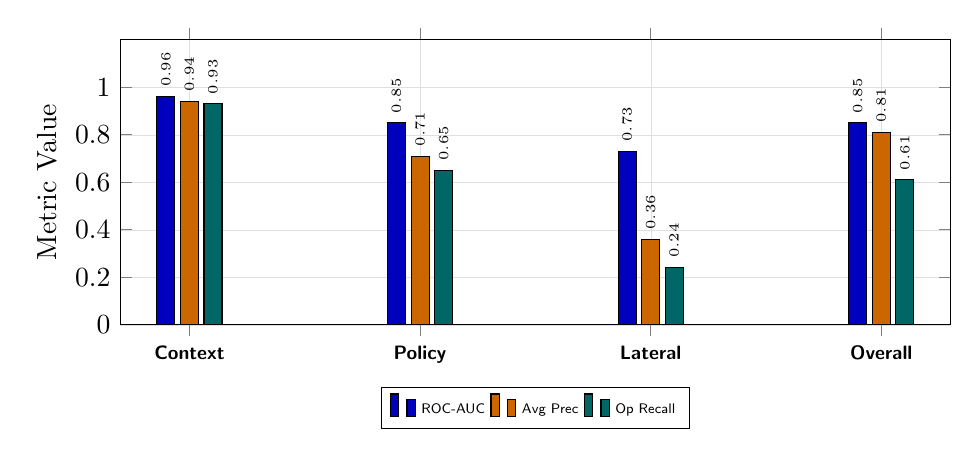
\begin{tikzpicture}
\begin{axis}[
  ybar,
  bar width=6.5pt,
  width=\columnwidth,
  height=5.2cm,
  ymin=0, ymax=1.2,
  ytick={0,0.2,0.4,0.6,0.8,1.0},
  ylabel={Metric Value},
  symbolic x coords={Context, Policy, Lateral, Overall},
  xtick=data,
  nodes near coords,
  nodes near coords style={font=\sffamily\tiny},
  every node near coord/.append style={rotate=90, anchor=west},
  legend style={at={(0.5,-0.22)}, anchor=north, legend columns=3, font=\sffamily\tiny},
  grid=both,
  grid style={line width=.1pt, draw=gray!25},
  x tick label style={font=\sffamily\scriptsize\bfseries}
]
  \addplot [fill=blue!75!black] coordinates {(Context, 0.96) (Policy, 0.85) (Lateral, 0.73) (Overall, 0.85)};
  \addplot [fill=orange!80!black] coordinates {(Context, 0.94) (Policy, 0.71) (Lateral, 0.36) (Overall, 0.81)};
  \addplot [fill=teal!80!black] coordinates {(Context, 0.93) (Policy, 0.65) (Lateral, 0.24) (Overall, 0.61)};
  \legend{ROC-AUC, Avg Prec, Op Recall}
\end{axis}
\end{tikzpicture}
\caption{Multi-class detection performance of the 5-node TGN on the de-leaked synthetic ZTA stream.}
\label{fig:perf_bars}
\end{figure}

\subsection{The contribution of the configuration node}

\begin{table}[ht!]
\centering
\renewcommand{\arraystretch}{1.5}
\footnotesize
\setlength{\tabcolsep}{4pt}
\begin{tabular}{lccc}
\toprule
Metric & 4 nodes & \textit{5 nodes} & $\Delta$ \\
\midrule
Aggregate AUC        & \BaggAucIII & \BaggAucIV & \BaggAucD \\
Aggregate AP         & \BaggApIII  & \BaggApIV  & \BaggApD \\
Aggregate recall (routed) & \BaggRecIII & \BaggRecIV & \BaggRecD \\
Lateral AUC          & \BlatAucIII & \BlatAucIV & \BlatAucD \\
Lateral AP           & \BlatApIII  & \BlatApIV  & \BlatApD \\
Lateral recall (routed) & \BlatRecIII & \textit{\BlatRecIV} & \textit{\BlatRecD} \\
Benign FPR (routed)  & \BfprIII    & \BfprIV    & \BfprD \\
\bottomrule
\end{tabular}
\caption{4-node chain versus 5-node chain with the configuration node, same
stream (\PanelBsettings).}
\label{tab:panelb}
\end{table}

Table~\ref{tab:panelb} isolates the configuration node by ablating it on the same
stream under routed evaluation. The introduction of the configuration node yields consistent
improvements across ranking and detection metrics: aggregate AUC improves by \BaggAucD{}
(reaching \BaggAucIV), lateral AUC increases by \BlatAucD{} (from \BlatAucIII{} to \BlatAucIV),
and lateral Average Precision improves by \BlatApD. Operating recall on lateral movement
reaches \BlatRecIV{} at an operating benign false-positive rate of \BfprIV. In credential
theft scenarios, the configuration node enables credential-reuse detection reaching AUC
\TheftAucOn{} and recall \TheftRecOn{} ($n=\TheftN$ theft events); ablating the node drops
performance to AUC \TheftAucOff{} and recall \TheftRecOff{} (\TheftSettings).

Beyond empirical metrics, the primary contribution of the configuration node is structural
expressiveness: on a 4-node chain, credential reuse presents no anomalous edge. Adding
the configuration node allows the temporal graph attention layers to recognize novel client
fingerprints associated with familiar principals.

\subsection{Component ablation scope}

While Table~\ref{tab:panelb} quantifies the impact of the configuration node and Table~\ref{tab:baselines}
isolates recurrent temporal memory against a static GNN, granular multi-seed ablation deltas
for secondary components (such as hashed identity embeddings versus indexed lookups or
isolated structural cosine heads) involve substantial combinatorial sweeps across seeds.
Verified empirical claims are therefore restricted to the 5-node causal chain, the
external commit gate protocol, and the dynamic temporal memory mechanism.
